First of all, a set of criteria is formulated, to indicate what general properties are the most crucial. These criteria cobbled with the functions and the model, lets us define the component structure.

\subsubsection{Criteria}

The criteria are based on the context of the system and the system definition. This is done to determine which properties are the most important for the system, for further development, and organising development resources toward the most important parts of the system. The criteria are shown in Table \ref{Criteria}.

\begin{table}[htb]
\centering
\begin{tabular}{|l|c|c|c|c|c|} \hline
	  & \textbf{Very} & \textbf{Important} & \textbf{Less} & \textbf{Irrelevant} & \textbf{Easily Fulfilled} \\ \hline
	\textbf{Usable} &  &  & X &  & \\ \hline
	\textbf{Secure} &  &  &  & X &  \\ \hline
	\textbf{Efficient} &  &  & X &  &  \\ \hline
	\textbf{Correct} &  & X &  &  &  \\ \hline
	\textbf{Reliable} & X &  &  &  &  \\ \hline
	\textbf{Maintainable} &  &  & X &  &  \\ \hline
	\textbf{Testable} & X &  &  &  &  \\ \hline
	\textbf{Flexible} &  & X &  &  &  \\ \hline
	\textbf{Comprehensive} &  &  & X &  &  \\ \hline
	\textbf{Reuseable} &  &  &  & X &  \\ \hline
	\textbf{Portable} &  &  &  & X &  \\ \hline
	\textbf{Interoperable} &  & X &  &  &  \\ \hline
\end{tabular}
\caption{Criteria for the system}
\label{Criteria}
\end{table}

The properties indicated as very important are ‘Reliable’ and ‘Testable’. Reliable means that the system can perform its functions with precision, and reliably every time. This is important because the system is a recommendation system, which requires various algorithms to compare media and users, to generate these recommendations. This functionality is therefore nessecary for the system to work properly. Testable is the property that makes it possible for the system to be tested and thereby ensuring that the systems runs as intended. This is crucial because, with time, the algorithm is going to require adjustments, and additions, to enhance the performance of the algorithm.

The other three important properties, correct, flexible, and interoperable, is also significant. Correct as an extension to the reliable property, signifying the importance of the algorithm working as intended. Flexible as mentioned above is also importent for the ability to modify and improve the system. Interoperable is important since the system is dependent on external sources to feed it new media data.

\subsubsection{Components}

Components are the parts which make up the layers of the system and in this section, these components is going to be defined, connected, and represented in a diagram. The layers for this system is divided into four parts: User interface, functions, model, and external sources or servers. See Figure \ref{Components}.

\begin{figure}[htb]
\centering
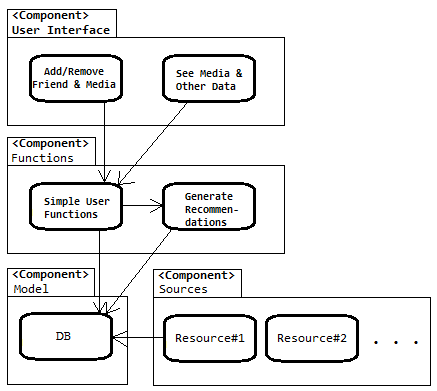
\includegraphics[width=0.7\textwidth]{Images/Components.png}
\caption{The components of the system, divided into layers}
\label{Components}
\end{figure}

The user interface layer contains everything that makes it possible for the user, to get access to and view data in the system. It has an add and remove component, for both media and friends, and a see component, which retrieves data from the system, making it viewable for the user.

Both of these are connected to a component in the functions layer, called ‘Simple user functions’. This component contains the procedures that retrieve data from the model and updates the model with data received from the user interface. This component is also connected to another component in the functions layer, called ‘Generate Recommendations’. As previously explained, this procedure is indirectly connected to the user and is activated through certain actions performed by the user, or by interval. Actions like the user logging into his account, or changing his preferences.

Both of these components are connected to the model, that contains all the concrete data regarding the users, media, and other notable classes and objects. It is represented by a component called DB, but will be updated in the forthcoming model component section \ref{ModelComponentSec}.

Using a server pattern, the last part of this component architecture is represented: External sources or servers. These are external servers and works together with the update media collections function. It is also through this function that these external sources are connected to the model layer of the component architecture.